\chapter{Learning}
\label{chapter:learning}

This chapter covers the learning part of this dissertation including data collecting, dataset preprocessing, and the models' structures and optimizations.

\section{Problem Introduction}

When anticipating the next action of the user, the object that the user is grasping can provide crucial information about the user's intention. Although an object detection algorithm may be helpful they can suffer from occlusion problems. Therefore, the following models attempt to solve this problem by taking an image of the user grasping a certain object and classifying which object is being grasped using the geometry of the hand.

To obtain a model that would be able to achieve the previous objective two experiments were made. In the first experiment, some types of models were tested with a smaller dataset containing only 300 images per object and 3 objects with the aim of knowing if they would be worth using and optimizing in a more complex problem. In the second experiment, a bigger dataset with 3000 images per object and 4 objects was used to train and optimize the models.

\section{Data Collecting}

The first step to train a supervised machine learning model is to find a dataset. However, given that this problem is very specific the datasets had to be manually collected. For this purpose, 2 datasets were collected with both consisting of a set of videos where one person would be moving and rotating a certain object. These videos were recorded at 10 frames per second to avoid consecutive frames having similar hand poses.

\textcolor{red}{image with examples from dataset}

In the first dataset, 3 different objects were used (see Fig: x), and for each one, 1 person was recorded for 30 seconds resulting in 300 images per object. In the second dataset, 4 objects were used (see Fig: x), and 3 people were recorded in 4 different 25-second videos for each object resulting in 1000 frames for each person and object making it 3000 frames for each object. Recording more than one video for each combination of person and object allowed each person to grasp the object slightly differently each time in order to obtain a more diverse dataset.

\textcolor{red}{image with objects}

\section{Dataset Preprocessing}

After having a dataset, the data had to be processed so that it would have a fitting structure to be used in the model training and testing. The images from the videos were processed using the Mediapipe hands model resulting in 21 points for each hand detected. The images were also processed by the full-body model also provided by Mediapipe so that it is possible to identify the right hand.

\textcolor{red}{image with examples from dataset with the points}

These points are then subject to further processing and normalization so that the location of the hand in the image and the distance between the hand and the camera have a lesser impact. The centroid is calculated and the points are translated so that they are centered in the (0.5, 0.5, 0.5) point, the points are then scaled up as much as possible while keeping every coordinate of every point between 0 and 1.

\textcolor{red}{2 images examples from dataset with the points and corresponding normalized points}

\section{Models}

\subsection{Convolutional Neural Network}

After all the processing, each sample provided to the model is made of the 21 points that represent the right hand. Given that points are related to each other, a one-dimensional convolutional neural network was used to take advantage of this characteristic. Therefore, the CNN is responsible for taking the 21 3D points and classifying the object that is being grasped.

\subsubsection{Initial Results}

Initially, a simple CNN was tested and manually optimized with the first dataset resulting in the following results:

\begin{minipage}{0.35\textwidth}
    \centering
    \captionof{table}{CNN Results in the First Dataset}
    \label{table:cnn_dataset1_results}
    \begin{tabular}{ |p{3.4cm}|p{1.1cm}| }
    \hline
    Metric & Value \\
    \hline
    Training Accuracy & 0.9813 \\
    \hline
    Validation Accuracy & 0.9775 \\
    \hline
    Test Accuracy & 0.9551 \\
    \hline
    Training Loss & 0.0493 \\
    \hline
    Validation Loss & 0.0794 \\
    \hline
    Test Loss & 0.1600 \\
    \hline
    Precision & 0.9583 \\
    \hline
    Recall & 0.9551 \\
    \hline
    F1-Score & 0.9549 \\
    \hline
    \end{tabular}
\end{minipage}%
\begin{minipage}{0.65\textwidth}
    \centering
    \includesvg[width=\textwidth, inkscapelatex=false]{figs/cnn_dataset1_conf_matrix.svg}
    \captionof{figure}[CNN Confusion Matrix in the First Dataset]{CNN Confusion Matrix in the First Dataset}
    \label{fig:cnn_confusion_matrix}
\end{minipage}

\if{0}
\begin{figure}
    \centering
    \def\svgwidth{\columnwidth}
    \input{figs/confusion_matrix.pdf_tex}
\end{figure}
\fi

\subsubsection{Final Model Architecture}

The model used is made of 2 convolutional layers followed by 3 dense layers with the third being the output layer. Between the convolutional and the dense layers and between both dense layers, there is also a dropout layer.

\begin{figure}[h]
\centerline{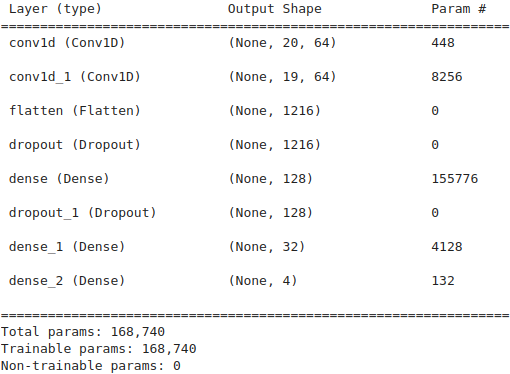
\includegraphics[height=3.4in]{figs/cnn_architecture.png}}
\caption[CNN Architecture]{CNN Model Architecture}
\label{fig:cnn_architecture}
\end{figure}

\subsubsection{Model Training}

In order to train the model, the dataset was split into 3 sets: the train set, the validation set, and the test set. Additionally, early stopping was set up so that the model would stop after 200 epochs without a better validation loss.

\subsubsection{Hyperparameter Optimization}

In this model, 4 hyperparameters were optimized to obtain better results. \textcolor{red}{explain why were these chosen}
These were:

\newcommand\myc{3cm}
\newcommand\mycc{7cm}
\newcommand\myccc{2.3cm}

\begin{table}[h!]
\caption{Hyperparameter Description and Tested Values}
\label{table:cnn_hyperparameters}
\centering
\begin{tabular}{ |p{\myc}|p{\mycc}|p{\myccc}| } 
\hline
Name & Description & Tested Values \\
\hline
\multirow{2}{\myc}{Learning Rate} & \multirow{2}{\mycc}{(learning rate description)} &\multirow{2}{\myccc}{0.01, 0.001, 0.0001} \\
& & \\
\hline
\multirow{3}{\myc}{Number of Convolutional Layers} & \multirow{3}{\mycc}{(Number of Convolutional Layers description)} & \multirow{3}{\myccc}{1, 2, 3} \\ 
& & \\
& & \\
\hline
\multirow{2}{\myc}{Kernel Size} & \multirow{2}{\mycc}{(kernel size description)} & \multirow{2}{\myccc}{2, 3} \\ 
& & \\
\hline
\multirow{2}{\myc}{Dropout Rate} & \multirow{2}{\mycc}{(dropout rate description)} & \multirow{2}{\myccc}{0.0, 0.1, 0.2, 0.3, 0.4, 0.5} \\ 
& & \\
\hline
\end{tabular}
\end{table}

\textcolor{red}{explain method for choosing}

\textcolor{red}{show best hyperparameters}

Best Hyperparameters: (lr, dr, ks, ncv) -> (0.001, 0.5, 3, 2)
Best Loss: 0.2095266580581665
Best Accuracy: 0.9415170103311539

\subsubsection{Final Results}

\begin{figure}[h]
\centerline{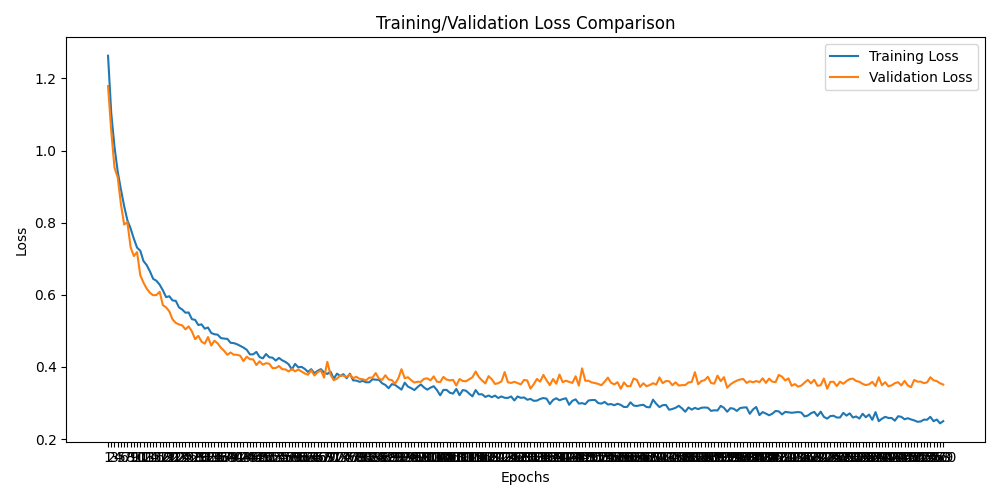
\includegraphics[width=14cm]{figs/loss_comparison.png}}
\caption[CNN training and validation loss evolution during training]{CNN training and validation loss evolution during training}
\label{fig:cnn_loss}
\end{figure}

\begin{figure}[h]
\centerline{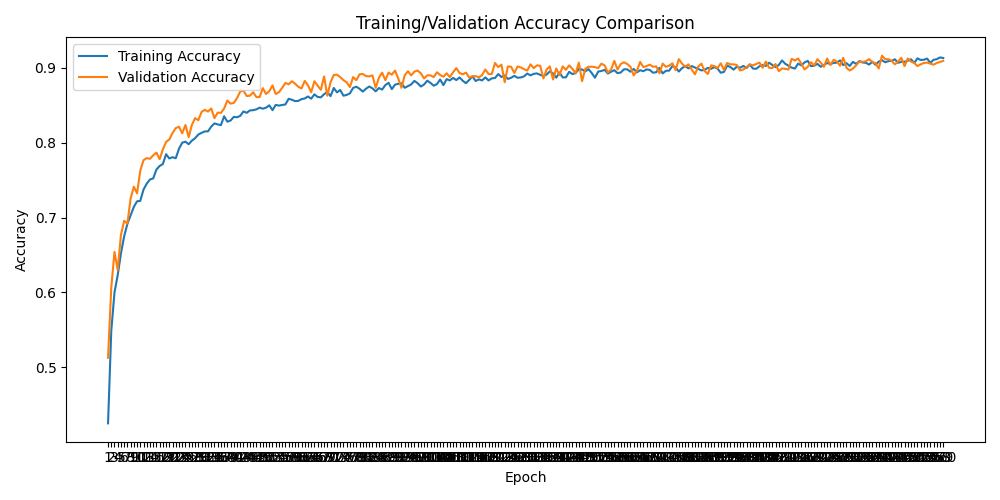
\includegraphics[width=14cm]{figs/acc_comparison.png}}
\caption[CNN training and validation accuracy evolution during training]{CNN training and validation accuracy evolution during training}
\label{fig:cnn_acc}
\end{figure}

\begin{figure}[h]
\centerline{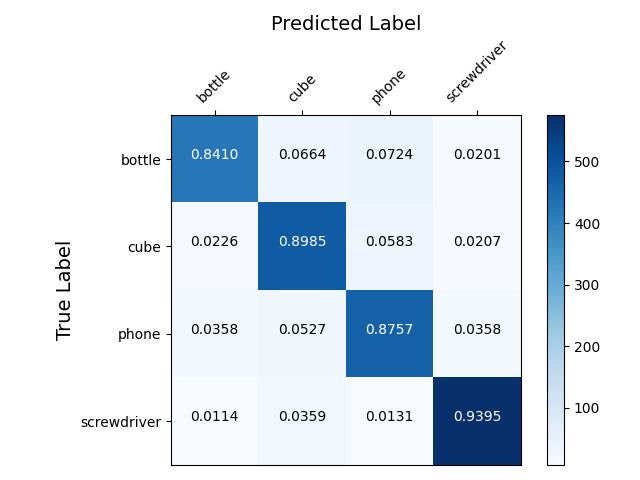
\includegraphics[width=12cm]{figs/conf_matrix.png}}
\caption[CNN confusion matrix]{CNN confusion matrix}
\label{fig:cnn_confusion_matrix}
\end{figure}

\subsection{Transformer Neural Network}

\subsubsection{Model Architecture}

\subsubsection{Model Training}

\subsubsection{Hyperparameter Optimization}

\subsubsection{Final Results}

\section{Models Comparison}

\subsection{All Users}

\subsection{One User}

\subsection{2 Train Users and 1 Test User}

\section{\textcolor{red}{Integration with Previous Work}}